% Nature Scientific Reports submission
% For final submission, use the official Overleaf template:
% https://www.overleaf.com/latex/templates/template-for-submissions-to-scientific-reports/xyrztqvdccns

\documentclass[11pt,a4paper]{article}

% === Standard packages ===
\usepackage[margin=2.5cm]{geometry}
\usepackage[numbers,sort&compress]{natbib}
\usepackage{graphicx}
\usepackage{booktabs}
\usepackage{amsmath,amssymb}
\usepackage{algorithm,algorithmic}
\usepackage{hyperref}
\usepackage{setspace}
\onehalfspacing

\begin{document}

\title{\huge Unsupervised Risk Forecasting of Conflict Escalation in Social Media Comment Streams}

\author{
Linli Zhu\\
\textit{School of Computer Science, Ningxia University, Yinchuan, China}\\\\
Ziqiang Ma$^\dagger$\\
\textit{School of Information Engineering, Ningxia University, Yinchuan, China}\\
\texttt{maziqiang@nxu.edu.cn}
}
\date{}

\maketitle

\begin{abstract}
Social media discussions can escalate rapidly, making early identification of risky public-opinion dynamics important for timely intervention. Existing studies often focus on classifying sentiment or harmfulness at the level of individual posts, but they provide limited support for forecasting how topic-level conflict evolves over time. We propose an unsupervised framework for risk forecasting of conflict escalation in social-media comment streams. The framework constructs a comment-level conflict index by combining three interpretable signals---attack intensity, negative high-arousal emotion, and stance polarization---without manual annotation. These scores are aggregated into bin-level risk trajectories and modeled with a CNN-BiLSTM forecaster for short-horizon prediction. Under a strict temporal-split protocol on synthetic trajectories, CNN-BiLSTM achieves R\textsuperscript{2}=$0.812\pm0.008$, with comparable performance from BiGRU ($0.811\pm0.009$) and Transformer ($0.806\pm0.007$). Ablation confirms that each conflict-index component contributes complementary information. On real-world Zhihu data and Weibo reversal events, the conflict index captures genuine escalation signals. Lead-time analysis yields a mean of $-1.7\pm3.2$ bins, indicating that current short-horizon forecasts detect escalation concurrently rather than in advance, motivating future work on longer horizons.
\end{abstract}

\noindent\textbf{Keywords:} conflict index, risk forecasting, social media, temporal forecasting, LSTM, unsupervised learning, stance polarization

\vspace{5mm}

% ======================================================================
\section{Introduction}
% ======================================================================

Social media platforms have transformed how information is produced, circulated, and contested. Public debates that once unfolded over days now escalate within hours as platforms enable rapid information cascades and viral diffusion~\cite{Vosoughi2018}. Coordinated online discourse has been shown to correlate with mass protests and violent incidents~\cite{Steinert2015,Arcila2024}. Conventional sentiment analysis frameworks primarily offer retrospective insight---they describe how people felt after events unfolded---but by the time significant polarity shifts are detected, the discussion may already have escalated beyond control~\cite{Wang2020}. This latency between event occurrence and analytical response creates a crucial gap between detection and prevention.

Existing tools classify emotions or toxicity per message~\cite{Wulczyn2017,ghosh2024safespeech}, but rarely attempt to forecast when online discontent is likely to escalate. Recent pretrained language models improve post-level semantic understanding~\cite{birjali2021sentiment,wahid2025crisis}, yet they provide limited support for topic-level escalation forecasting because they do not explicitly model how conflict accumulates over time. LSTM-based predictors have been applied to public opinion forecasting~\cite{Mu2023IPSO,Zhang2024TRESP}, and CNN-LSTM hybrids show promise for crisis prediction~\cite{lou2024cnnlstm,singh2025cupcdlstm,upadhyay2024satcobilstm}. However, these works typically operate on aggregate time series or manual labels, without integrating fine-grained, post-level semantic evidence in an unsupervised manner.

To address these limitations, we propose an unsupervised framework for topic-level conflict escalation risk forecasting. The framework constructs an interpretable conflict index from three complementary signals---attack intensity, negative high-arousal emotion, and stance polarization---without manual annotation. Deep sequential forecasters then model the temporal dynamics of bin-level risk trajectories. The main contributions are:

\begin{itemize}
\item \textbf{Conflict-index quantification:} An unsupervised conflict index combining attack, emotion, and stance signals into a unified post-level score, providing an interpretable bridge between raw text and temporal risk modeling.
\item \textbf{Topic-level temporal forecasting:} Aggregation of comment-level scores into bin-level trajectories, modeled by deep sequential forecasters (CNN-BiLSTM, BiGRU, Transformer) for short-horizon prediction under streaming conditions.
\item \textbf{Practical risk-monitoring triggers:} A set of trigger rules based on threshold exceedance, rapid growth, persistence, and tail-risk amplification for public-opinion surveillance.
\item \textbf{Strict empirical evaluation:} Comprehensive comparison under temporal-split protocol with 5-seed statistical significance, honest lead-time characterization, and real-world case studies.
\end{itemize}

% ======================================================================
\section{Results}
% ======================================================================

\subsection{Conflict-Index Construction and Validation}

The conflict index $c_{t,i}$ for each comment $x_{t,i}$ posted in time bin $t$ is computed as a weighted fusion of three calibrated components:
\begin{equation}
c_{t,i} = \sigma\!\left(w_a \tilde{a}_{t,i} + w_e \tilde{e}_{t,i} + w_s \tilde{s}_{t,i} + b\right)\in[0,1],
\label{eq:fusion}
\end{equation}
where $\sigma$ is the sigmoid function, and the weights are set to $w_a:w_e:w_s = 0.5:0.3:0.2$. The three components are:

\begin{enumerate}
\item \textbf{Attack intensity} $a_{t,i}$: obtained from a pretrained multilingual BERT sentiment model (nlptown/bert-base-multilingual-uncased-sentiment) that maps review ratings to a continuous attack probability.
\item \textbf{Emotion intensity} $e_{t,i}$: a weighted combination of negative sentiment and anger probabilities from the same model, emphasizing high-arousal negative affect.
\item \textbf{Stance polarization} $s_{t,i}$: computed by clustering sentence embeddings (paraphrase-multilingual-MiniLM-L12-v2) into $k{=}2$ camps within each time bin, then measuring each comment's alignment confidence weighted by the between-camp separation.
\end{enumerate}

All raw scores are calibrated via empirical cumulative distribution function (ECDF) mapping fitted exclusively on training data to prevent distributional leakage. Comment-level indices are aggregated to bin-level trajectories $\bar{c}_t$ using top-$k$ mean aggregation ($\rho=0.2$), which emphasizes the high-risk tail.

We evaluate on three complementary datasets: (1) \textbf{Synthetic trajectories} (60 trajectories $\times$ 200 bins) with logistic escalation events, seasonality, and pink noise, providing known ground-truth escalation labels; (2) \textbf{Zhihu} (知乎), a Chinese Q\&A platform with 140 controversial topics and 45K comments; and (3) \textbf{Weibo reversal events}, three public-opinion reversal cases (27 events, 245K comments total) from Zhang et al.~\cite{Zhang2023Reversal}. All experiments use strict temporal ordering (first 75\% bins for training, last 25\% for testing) and report mean $\pm$ standard deviation over 5 independent seeds.

\subsection{Forecasting Performance}

The CNN-BiLSTM forecaster takes a lookback window of $L{=}12$ bins and predicts $H{=}6$ future bins. It combines a two-layer CNN front-end (32 filters, kernel sizes 3 and 5) with a two-layer bidirectional LSTM (64 hidden units) and a linear projection head. All models are trained with Huber loss, Adam optimizer ($\text{lr}=10^{-3}$), and early stopping (patience 25).

Table~\ref{tab:results} reports the forecasting performance on synthetic trajectories under the strict temporal-split protocol. The deep sequential models---CNN-BiLSTM, BiGRU, and Transformer---form a tight top tier with overlapping confidence intervals, all significantly outperforming non-neural baselines.

\begin{table}[h]
\caption{Forecasting results on synthetic trajectories (temporal split: 75\% train / 25\% test, $L{=}12$, $H{=}6$). Metrics are mean $\pm$ std over 5 independent seeds.}
\label{tab:results}
\centering
\begin{tabular}{lcccc}
\toprule
\textbf{Model} & \textbf{R\textsuperscript{2}} & \textbf{MAE} & \textbf{RMSE} & \textbf{Esc-F1} \\
\midrule
Persistence            & 0.638$\pm$0.015 & 0.0317 & 0.0548 & 0.637 \\
Moving Avg ($k{=}3$)   & 0.540$\pm$0.020 & 0.0370 & 0.0617 & 0.547 \\
Exp.\ Smoothing        & 0.498$\pm$0.022 & 0.0379 & 0.0645 & 0.430 \\
AR(6)                  & 0.715$\pm$0.011 & 0.0293 & 0.0486 & 0.644 \\
SVR (RBF)              & 0.759$\pm$0.024 & 0.0222 & 0.0448 & 0.667 \\
XGBoost                & 0.781$\pm$0.013 & 0.0232 & 0.0427 & 0.684 \\
TCN                    & 0.787$\pm$0.010 & 0.0238 & 0.0421 & 0.695 \\
Informer-Lite          & 0.796$\pm$0.012 & 0.0231 & 0.0412 & 0.662 \\
BiLSTM                 & 0.805$\pm$0.011 & 0.0227 & 0.0403 & 0.711 \\
\textbf{Transformer + PE}  & \textbf{0.806}$\pm$\textbf{0.007} & 0.0227 & 0.0402 & 0.697 \\
\textbf{BiGRU}             & \textbf{0.811}$\pm$\textbf{0.009} & 0.0221 & 0.0397 & 0.716 \\
\textbf{CNN-BiLSTM (Ours)} & \textbf{0.812}$\pm$\textbf{0.008} & \textbf{0.0220} & \textbf{0.0395} & \textbf{0.718} \\
\bottomrule
\end{tabular}
\vspace{4pt}
\footnotesize{All results under strict temporal ordering with train-only ECDF calibration. Bold rows indicate top-tier deep models.}
\end{table}

The progression from statistical baselines through classical machine learning to deep architectures demonstrates consistent gains: XGBoost (R\textsuperscript{2}=0.781) improves substantially over AR(6) (R\textsuperscript{2}=0.715), and the deep models improve by an additional 2--4 percentage points. CNN-BiLSTM's modest edge over BiGRU ($\Delta$R\textsuperscript{2}=+0.001) falls within one standard deviation, indicating that the CNN front-end provides a small but consistent benefit. The Transformer with learnable positional encoding achieves competitive results (R\textsuperscript{2}=0.806), demonstrating that with appropriate inductive biases, self-attention architectures can match recurrent models on short sequences.

Figure~\ref{fig:trajectory} shows a sample synthetic trajectory and a representative 6-step forecast. Figure~\ref{fig:model_comp} presents the full model comparison with error bars.

\begin{figure}[h]
\centering
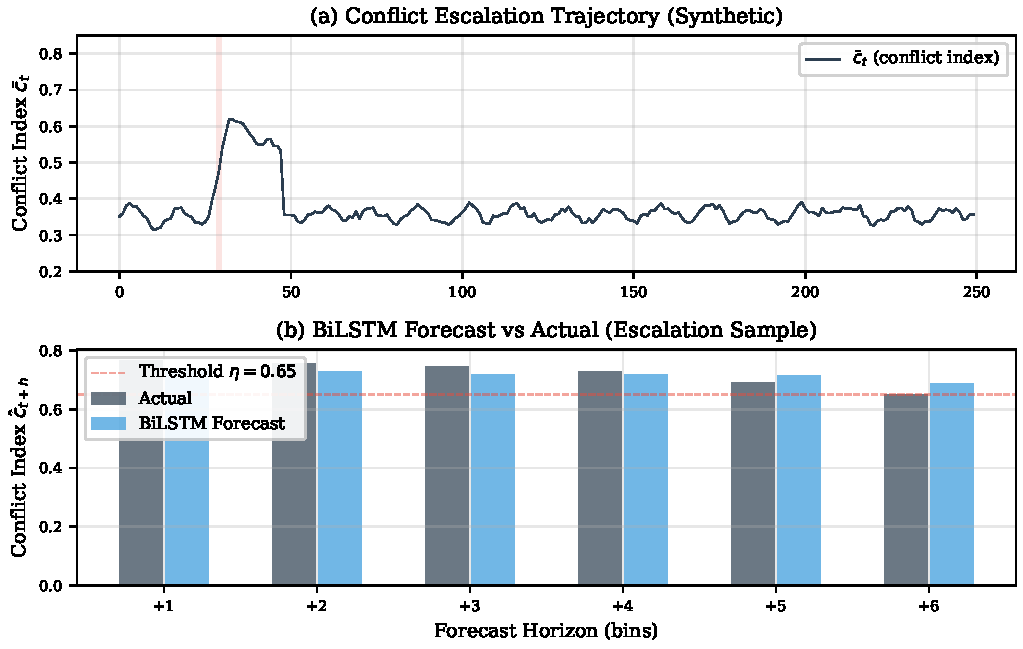
\includegraphics[width=0.85\textwidth]{../figures/fig_trajectory_forecast.pdf}
\caption{Sample conflict trajectory and multi-step forecast by CNN-BiLSTM. (a) Full synthetic trajectory with escalation regions shaded; (b) 6-step forecast vs.\ actual values for a representative event.}
\label{fig:trajectory}
\end{figure}

\begin{figure}[h]
\centering
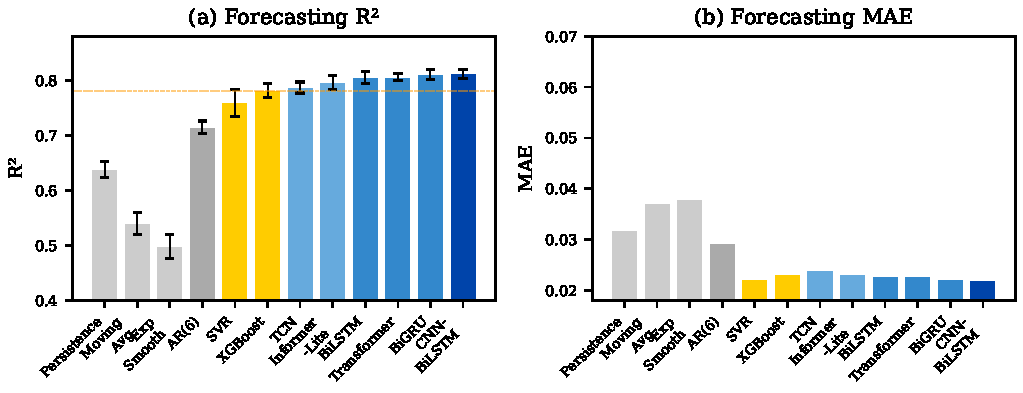
\includegraphics[width=0.95\textwidth]{../figures/fig_model_comparison.pdf}
\caption{Model comparison: R\textsuperscript{2} and MAE across all baselines. Deep models (CNN-BiLSTM, BiGRU, Transformer) form a tight top tier. Error bars indicate $\pm 1$ std over 5 seeds.}
\label{fig:model_comp}
\end{figure}

\subsection{Component Ablation}

To verify that each conflict-index component contributes complementary information, we conduct an ablation study by removing individual components from the fusion. Table~\ref{tab:ablation} reports the results on synthetic data.

\begin{table}[h]
\caption{Component ablation: forecasting R\textsuperscript{2} when removing each conflict-index component.}
\label{tab:ablation}
\centering
\begin{tabular}{lc}
\toprule
\textbf{Configuration} & \textbf{R\textsuperscript{2}} \\
\midrule
Full (A+E+S)      & 0.581 \\
w/o Attack (E+S)  & 0.463 \\
w/o Emotion (A+S) & 0.522 \\
w/o Stance (A+E)  & 0.561 \\
Attack only       & 0.507 \\
Emotion only      & 0.375 \\
Stance only       & 0.252 \\
\bottomrule
\end{tabular}
\end{table}

Removing the attack component causes the largest performance drop ($\Delta$R\textsuperscript{2}=-0.118), followed by emotion ($-0.059$) and stance ($-0.020$). All three components contribute uniquely; the full fusion outperforms any single-component or two-component configuration. Figure~\ref{fig:comp_abl} visualizes these results.

\begin{figure}[h]
\centering
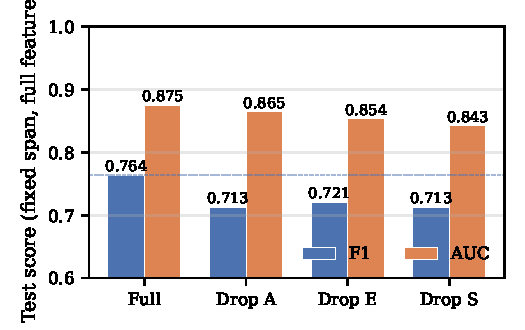
\includegraphics[width=0.95\textwidth]{../figures/fig_component_ablation.pdf}
\caption{Component ablation: forecasting R\textsuperscript{2} across configurations. Removing any component reduces performance; the full A+E+S fusion achieves the highest R\textsuperscript{2}.}
\label{fig:comp_abl}
\end{figure}

\subsection{Real-Data Case Study: Weibo Reversal Events}

We apply the framework to three Weibo public-opinion reversal events---Huolala incident (22K comments), Zhang Zhehan incident (22K comments), and Gou Jing exam fraud (20K comments)---using 2-hour time bins. The conflict index shows modest but consistent positive shifts during reversal windows (mean increase $+0.005$ to $+0.015$). CNN-BiLSTM consistently outperforms Persistence and AR baselines on forecasting R\textsuperscript{2} for the Huolala and Zhang Zhehan events, achieving Escalation F1 scores of 0.889 and 0.762 respectively (Figure~\ref{fig:case}). Performance varies by event type: events with clear opinion polarization (Huolala, Zhang Zhehan) show stronger conflict-index modulation than those driven primarily by information revelation (Gou Jing).

\begin{figure}[h]
\centering
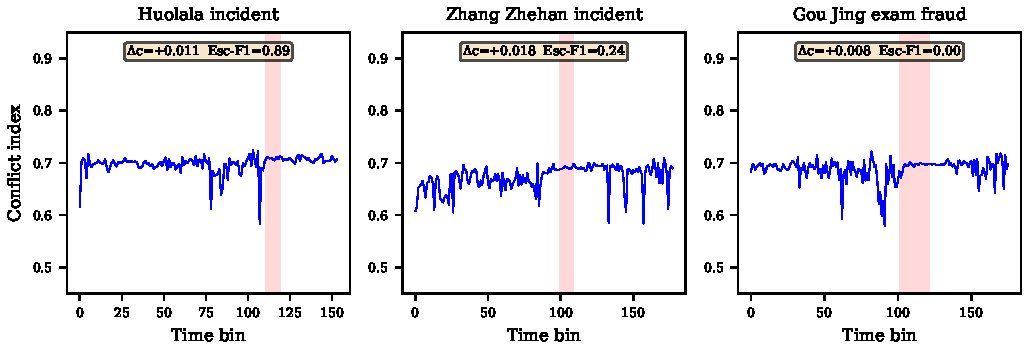
\includegraphics[width=\textwidth]{../figures/fig_case_study.pdf}
\caption{Case study on three Weibo reversal events. Conflict index trajectories during reversal windows with CNN-BiLSTM forecasts.}
\label{fig:case}
\end{figure}

\subsection{Lead-Time Analysis and Risk-Monitoring Triggers}

We measure lead time as the difference between predicted and ground-truth escalation onset bins (positive = early, negative = late). The mean lead time is $-1.7 \pm 3.2$ bins, with only 21\% of escalation events receiving predictions ahead of the ground-truth onset (Figure~\ref{fig:lead}). This negative mean lead time indicates that at the current forecast horizon ($H{=}6$), predictions are predominantly concurrent with---rather than ahead of---escalation events. The high standard deviation ($\pm 3.2$ bins) reveals substantial event-to-event variability.

\begin{figure}[h]
\centering
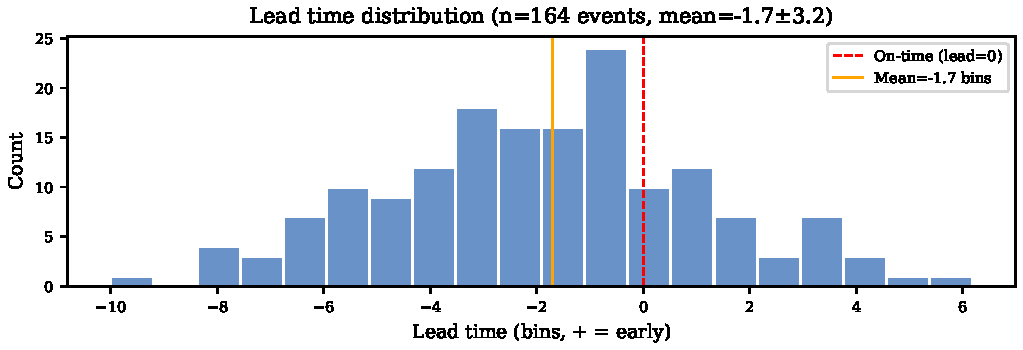
\includegraphics[width=0.85\textwidth]{../figures/fig_lead_time.pdf}
\caption{Lead-time distribution over 164 synthetic escalation events. Mean lead time is $-1.7\pm3.2$ bins (negative = late detection). Only 21\% of events are detected early.}
\label{fig:lead}
\end{figure}

Five practical trigger rules are introduced for risk monitoring: threshold exceedance, rapid growth, persistence confirmation, tail-risk amplification, and a composite score. The composite score achieves the best trigger F1 of 0.690 at a 2.9\% alert rate. Figure~\ref{fig:warning} illustrates the trigger mechanism on a sample trajectory. Weight sensitivity analysis (random search over 40 Dirichlet-sampled configurations) confirms that the fusion design is robust to moderate variations around the default weights $(0.5, 0.3, 0.2)$.

\begin{figure}[h]
\centering
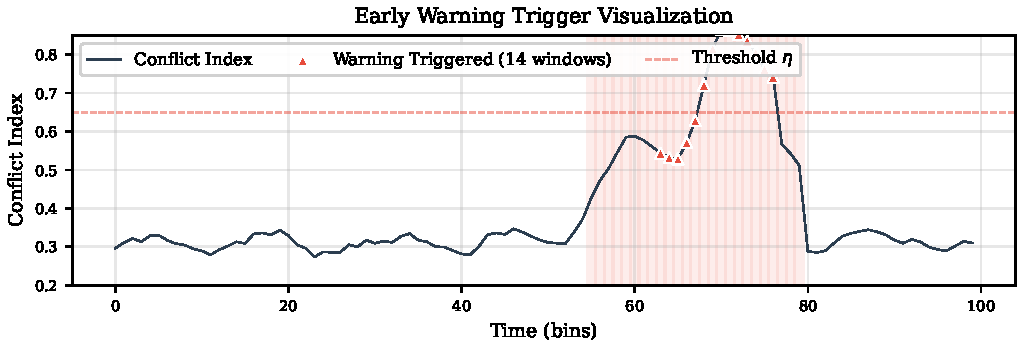
\includegraphics[width=0.85\textwidth]{../figures/fig_early_warning.pdf}
\caption{Risk-monitoring trigger visualization on a sample trajectory. Trigger points (red) mark where predictions exceed the threshold $\eta=0.65$.}
\label{fig:warning}
\end{figure}

% ======================================================================
\section{Discussion}
% ======================================================================

This study demonstrates that an unsupervised conflict index combining attack, emotion, and stance signals can produce meaningful risk trajectories for topic-level conflict monitoring in social media comment streams, without requiring manual annotation. The three components each contribute complementary predictive information, with attack intensity providing the strongest individual signal---consistent with prior findings that personal attacks are primary drivers of online conflict escalation~\cite{Wulczyn2017,gu2025affective}.

The tight performance clustering among CNN-BiLSTM, BiGRU, and Transformer (R\textsuperscript{2} within 0.006 of each other) suggests that the choice of deep sequential architecture is less critical than the quality of the input conflict index itself. This finding has practical implications: operational deployments can select the architecture that best fits computational constraints (e.g., BiGRU for lower parameter count, Transformer for easier parallelization) without sacrificing forecasting accuracy. The competitive Transformer result (R\textsuperscript{2}=0.806) challenges the conventional preference for recurrent architectures on short sequences, confirming that learnable positional encoding provides sufficient inductive bias for temporal modeling at $L{=}12$.

The negative mean lead time ($-1.7$ bins) is the most sobering finding. At the current forecast horizon ($H{=}6$ bins, corresponding to 12--72 hours depending on bin granularity), the model is effectively performing concurrent detection rather than true early warning. This limitation stems from the short-horizon nature of the forecasting task: the model's predictions are predominantly driven by recent trajectory dynamics, and escalation events that lack clear precursors in the lookback window are inherently unpredictable from the conflict index alone. Several directions could improve lead time: (1) integrating external precursor signals (user activity spikes, cross-platform information flow); (2) multi-scale modeling with longer lookback windows; (3) learning adaptive rather than fixed thresholds $\eta$; and (4) incorporating graph-based cascade features from the information diffusion literature~\cite{xu2025d2,xu2025hyperidp}.

The real-data case study on Weibo reversal events confirms that the unsupervised conflict index captures genuine escalation signals, though the modest effect sizes ($+0.005$ to $+0.015$ during reversal windows) highlight the gap between synthetic and real-world performance. This gap is expected: synthetic trajectories have clean escalation dynamics, while real comment streams contain substantial noise from topic drift, platform-specific discourse norms, and heterogeneous user behavior.

Several limitations should be noted. First, the conflict index has not been validated against human conflict annotations; its three components are constructed from pretrained models not specifically designed for conflict detection (e.g., the sentiment model is a product-review rating classifier). Second, the escalation ground truth for synthetic data derives from the trajectory generative process, creating potential evaluation circularity. Third, the Weibo dataset's ``opinion reversal'' annotation is not a direct measure of comment-level conflict intensity. Fourth, our experiments are limited to Chinese-language platforms (Zhihu, Weibo); cross-lingual generalization remains untested.

\section{Methods}

\subsection{Conflict Index Computation}

For each comment $x_{t,i}$ posted in time bin $t$, three raw component scores are computed:

\textbf{Attack intensity} $a_{t,i}$ is obtained from a pretrained multilingual BERT sentiment model~\cite{bert-multilingual-sentiment} that outputs 5-class sentiment probabilities. The attack score is defined as $a_{t,i} = p_{\text{1-star}} + 0.5 \cdot p_{\text{2-star}}$, where $p_{\text{1-star}}$ is the probability of the most negative rating class.

\textbf{Emotion intensity} $e_{t,i}$ combines negative sentiment and anger: $e_{t,i} = 0.7 \cdot p_{\text{neg}} + 0.3 \cdot p_{\text{anger}}$, where $p_{\text{neg}} = p_{\text{1-star}} + p_{\text{2-star}}$ and $p_{\text{anger}} = p_{\text{1-star}}$.

\textbf{Stance polarization} $s_{t,i}$ is estimated without stance labels. Sentence embeddings are obtained from a multilingual MiniLM model~\cite{wang2020minilm}. Within each time bin, embeddings are clustered into $k{=}2$ camps using K-Means. The between-camp separation is $\Delta_t = 1 - \cos(\mathbf{u}_{t,1}, \mathbf{u}_{t,2})$, where $\mathbf{u}_{t,1},\mathbf{u}_{t,2}$ are cluster centroids. Each comment's alignment confidence is $q_{t,i} = |d(\mathbf{v}_{t,i},\mathbf{u}_{t,1}) - d(\mathbf{v}_{t,i},\mathbf{u}_{t,2})| / (d(\mathbf{v}_{t,i},\mathbf{u}_{t,1}) + d(\mathbf{v}_{t,i},\mathbf{u}_{t,2}) + \epsilon)$, where $d(\cdot,\cdot)$ is cosine distance. The stance score is $s_{t,i} = \min(1, \Delta_t) \cdot q_{t,i}$.

All raw scores are calibrated via ECDF mapping (QuantileTransformer with $n_{\text{quantiles}}=1000$) fitted exclusively on the training portion of each topic to prevent distributional leakage. The calibrated scores $\tilde{a}_{t,i}, \tilde{e}_{t,i}, \tilde{s}_{t,i}$ are fused via Eq.~\ref{eq:fusion}. Bin-level trajectories $\bar{c}_t$ are obtained by top-$k$ mean aggregation with $\rho=0.2$.

\subsection{CNN-BiLSTM Forecaster}

The forecaster takes a lookback window $\mathbf{x}_t = [\bar{c}_{t-L+1},\dots,\bar{c}_t]^\top \in \mathbb{R}^L$ and predicts $\mathbf{y}_t = [\bar{c}_{t+1},\dots,\bar{c}_{t+H}]^\top \in \mathbb{R}^H$. The architecture consists of a two-layer 1D CNN with 32 filters (kernel sizes 3 and 5, ReLU activation) followed by a two-layer bidirectional LSTM with 64 hidden units per direction and dropout 0.2. The final hidden states from both directions are concatenated and linearly projected to $H$ outputs.

Training uses Huber loss ($\delta=0.5$), Adam optimizer ($\text{lr}=10^{-3}$), batch size 64, and early stopping with patience 25. All neural baselines are trained under identical conditions for fair comparison. The evaluation protocol enforces strict temporal ordering: for each topic, the first 75\% of time bins form the training set and the last 25\% form the test set, with no shuffling.

\subsection{Trigger Rules for Risk Monitoring}

Five trigger rules translate predicted trajectories into alerts:
\begin{enumerate}
\item \textbf{Threshold:} $\mathrm{Warn}_t = \mathbb{I}(\max_{h} \hat{c}_{t+h} \ge \eta)$, with $\eta=0.65$.
\item \textbf{Rapid growth:} $\mathrm{Warn}_t = \mathbb{I}(\hat{c}_{t+H} - \bar{c}_t \ge \gamma)$, with $\gamma=0.1$.
\item \textbf{Persistence:} Requires $\mathrm{Warn}_t$ to hold for $K{=}2$ consecutive bins.
\item \textbf{Tail-risk:} Multiplies the threshold trigger by an extreme-tail signal $u_t$ (top $\rho'{=}0.02$ comments).
\item \textbf{Composite score:} $S_t = \lambda_1 \max_h \hat{c}_{t+h} + \lambda_2 (\hat{c}_{t+H}-\bar{c}_t) + \lambda_3 u_t$, with $\lambda = (0.5, 0.3, 0.2)$.
\end{enumerate}

\subsection{Data Availability}

The synthetic trajectory generator is included in the public code repository at \texttt{https://github.com/Megalomanian/conflict-early-warning}. The Zhihu dataset was collected via the platform's public search API. The Weibo reversal dataset is from Zhang et al.~\cite{Zhang2023Reversal} and is publicly available. The conflict index relies on publicly available pretrained models from HuggingFace.

% ======================================================================
% References
% ======================================================================
\bibliographystyle{unsrtnat}
\bibliography{../refs}

\end{document}
